\documentclass[letterpaper,11pt]{article}
\usepackage{xeCJK}
\usepackage{bm}
\usepackage{geometry}
\usepackage{amssymb}
\usepackage{amsmath}
\usepackage[cal=boondoxo, scr=dutchcal]{mathalfa}
\usepackage{multirow}
\usepackage[unicode, CJKbookmarks=true]{hyperref}

\numberwithin{equation}{section}

\geometry{a4paper,left=2cm,right=2cm,top=2cm,bottom=2cm}

\usepackage{setspace}
\setstretch{1.1}
\setlength{\parskip}{0.1\baselineskip}

\usepackage{graphicx}
\usepackage{caption}

\begin{document}

\title{变换矩阵}
\author{张驰}
\maketitle

\section{3D线性变换}

\begin{figure}
    \begin{center}
        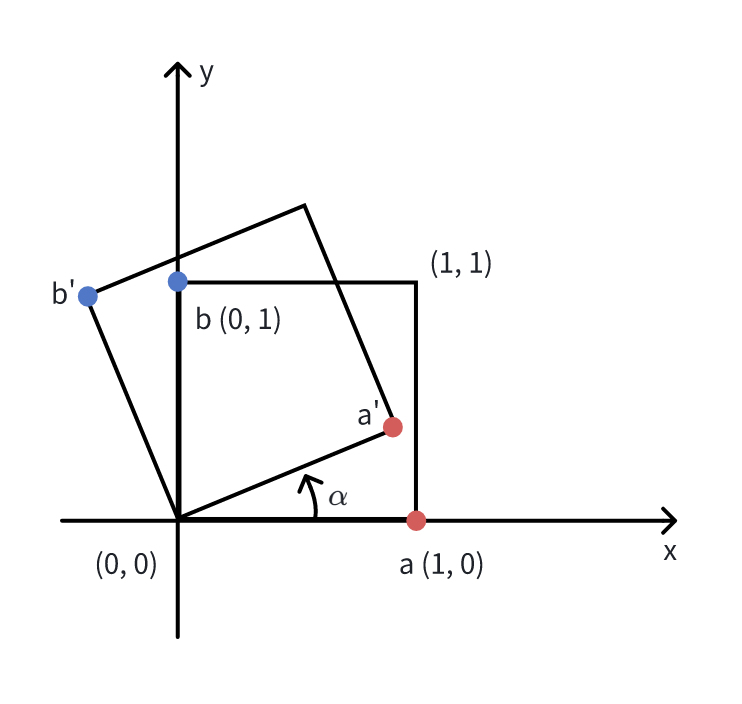
\includegraphics[width=0.5\textwidth]{imgs/2d-rotate.png}
    \end{center}
    \caption{\label{fig:2d-rotate}2维空间旋转}
\end{figure}

\end{document}
